% =============================================================================
% Chapter 4: Agent Communication Protocol
% פרוטוקול התקשורת בין סוכנים
% Based on original Chapter 7
% =============================================================================

\documentclass[../master/main.tex]{subfiles}

\begin{document}

\setcounter{chapter}{3}
\hebrewchapter{פרוטוקול התקשורת בין סוכנים}
\hebrewchapterlabel{chap:protocol}

\par\needspace{5\baselineskip}
\hebrewsection{מבוא}

פרק זה מתמקד בפרוטוקול התקשורת \protocol{} המאפשר לסוכנים לתקשר זה עם זה באופן אמין ומסודר. הפרוטוקול מבוסס על עקרונות של תקשורת סוכנים פתוחה: הודעות ממוסגרות היטב, שדות חובה ורשות, זיהוי שיחות, וסטטוס חד-ערכי.

\par\needspace{4\baselineskip}
\hebrewsubsection{מטרות הפרק}

בסיום פרק זה, תבינו:
\begin{itemize}
    \item את שכבת התעבורה מבוססת \gmailapi{}
    \item את מבנה המעטפה (\en{Envelope}) עם הכותרת המשותפת
    \item את סוגי ההודעות השונים
    \item את חובת ה-\en{CC} לשרת הלוג
    \item את מערכת המועדים וניהול הזמנים
\end{itemize}

% =============================================================================
\par\needspace{5\baselineskip}
\hebrewsection{שכבת התעבורה --- \gmailapi{}}
\label{sec:gmail-transport}
% =============================================================================

\par\needspace{4\baselineskip}
\hebrewsubsection{הרעיון המרכזי}

בניגוד לארכיטקטורות מסורתיות המשתמשות בשרתי \en{HTTP}, מערכת הליגה משתמשת ב-\gmailapi{} כשכבת תעבורה.

\textbf{יתרונות הבחירה:}
\begin{itemize}
    \item \textbf{ללא צורך בשרת} --- הסוכנים פועלים כתהליכים עצמאיים
    \item \textbf{תקשורת אסינכרונית} --- הודעות נשמרות עד לעיבוד
    \item \textbf{דיבוג פשוט} --- כל הודעה נשמרת באינבוקס
    \item \textbf{``הילוך איטי''} --- קל לעקוב ולהבין מה קורה
    \item \textbf{אמינות מובנית} --- \en{Gmail} מספק אמינות גבוהה
\end{itemize}

\needspace{10\baselineskip}
\begin{notebox}[\hebtitle{מגבלות \en{Gmail API}}]
חשוב להכיר את מגבלות \en{Gmail API} לפני המימוש: חשבון חינמי מוגבל ל-\num{500} הודעות ליום, עם מגבלות קצב של \num{250} יחידות מכסה לשנייה. לניתוח מפורט של המגבלות והתאמתן לתעבורת הליגה, ראו נספח~ה' (עמ'~\pageref{sec:gmail-api-limits}).
\end{notebox}

\par\needspace{4\baselineskip}
\hebrewsubsection{הקבלה ל-\en{HTTP}}

טבלה~\ref{tab:http-gmail-comparison} מציגה את ההקבלות בין \en{HTTP} ל-\en{Gmail}.

\begin{fancytable}{R{3cm}cR{3cm}}{השוואה בין \en{HTTP} ל-\en{Gmail}}
\label{tab:http-gmail-comparison}
\en{Gmail} & \en{HTTP} & פעולה \\
שליחת אימייל & \en{\texttt{POST /endpoint}} & שליחת הודעה \\
קריאת אימייל & \en{\texttt{GET /endpoint}} & קבלת הודעה \\
\en{JSON attachment} & \en{JSON in body} & גוף ההודעה \\
כתובת מייל & \en{URL} & כתובת יעד \\
\end{fancytable}

\par\needspace{4\baselineskip}
\hebrewsubsection{מבנה הודעת \en{Gmail}}

כל הודעה נשלחת עם המבנה הבא:

\begin{itemize}
    \item \textbf{\en{From}} --- כתובת הסוכן השולח
    \item \textbf{\en{To}} --- כתובת הסוכן המקבל
    \item \textbf{\en{CC}} --- \textbf{חובה}: שרת הלוג
    \item \textbf{\en{Subject}} --- מזהה פרוטוקול והודעה
    \item \textbf{\en{Attachment}} --- קובץ \en{JSON} עם תוכן ההודעה
\end{itemize}

% =============================================================================
\par\needspace{5\baselineskip}
\hebrewsection{פורמט נושא האימייל}
\label{sec:email-subject-format}
% =============================================================================

\par\needspace{4\baselineskip}
\hebrewsubsection{מבנה הנושא}

כל אימייל בפרוטוקול כולל נושא (\en{Subject}) בפורמט מוגדר:

\begin{english}
\begin{lstlisting}[basicstyle=\ttfamily\small,breaklines=true]
league.v2::<ROLE>::<EMAIL>::<TXID>::<MESSAGETYPE>
\end{lstlisting}
\end{english}

\begin{fancytable}{lHH}{רכיבי נושא האימייל}
\label{tab:subject-components}
רכיב & תיאור & דוגמה \\
\en{protocol} & גרסת הפרוטוקול & \en{league.v2} \\
\en{ROLE} & תפקיד השולח & \en{PLAYER}, \en{REFEREE}, \en{LEAGUEMANAGER} \\
\en{EMAIL} & כתובת השולח & \en{mygroup.player@gmail.com} \\
\en{TXID} & מזהה טרנזקציה & \en{tx-20260113-abc123} \\
\en{MESSAGETYPE} & סוג ההודעה & \en{LEAGUEREGISTERREQUEST} \\
\end{fancytable}

\par\needspace{4\baselineskip}
\hebrewsubsection{דוגמאות לנושאי אימייל}

\begin{english}
\begin{pythonbox}[\hebtitle{דוגמאות לנושאי אימייל}]
# Player registration request
league.v2::PLAYER::mygroup.player@gmail.com::tx-20260113-abc::LEAGUEREGISTERREQUEST

# Referee registration request
league.v2::REFEREE::mygroup.referee@gmail.com::tx-20260113-def::REFEREEREGISTERREQUEST

# Broadcast from League Manager
league.v2::LEAGUEMANAGER::bitalevi100@gmail.com::bc-550e8400::BROADCAST_KEEP_ALIVE

# Game invitation from referee
league.v2::REFEREE::mygroup.referee@gmail.com::tx-20260117-ghi::GAMEINVITATION
\end{pythonbox}
\end{english}

\needspace{8\baselineskip}
\begin{implementationbox}
\textbf{פירוק נושא האימייל בקוד:}

\begin{english}
\begin{lstlisting}[basicstyle=\ttfamily\small,breaklines=true,language=Python]
def parse_subject(subject: str) -> dict:
    parts = subject.split("::")
    return {
        "protocol": parts[0],    # "league.v2"
        "role": parts[1],        # "PLAYER" / "REFEREE" / "LEAGUEMANAGER"
        "email": parts[2],       # sender email
        "txid": parts[3],        # transaction ID
        "message_type": parts[4] # message type
    }
\end{lstlisting}
\end{english}
\end{implementationbox}

% =============================================================================
\par\needspace{5\baselineskip}
\hebrewsection{מבנה המעטפה --- \en{Shared Header}}
\label{sec:envelope}
% =============================================================================

\par\needspace{10\baselineskip}
\hebrewsubsection{שדות הכותרת המשותפת}

\needspace{6\baselineskip}
\begin{notebox}[\hebtitle{פורמט ההודעות --- קובץ \en{JSON}}]
\textbf{חשוב לזכור:} כל הודעה בפרוטוקול נשלחת כ\textbf{קובץ \en{JSON} מצורף לאימייל}. גוף האימייל עצמו יכול להיות ריק או להכיל תקציר קריא לאדם, אך \textbf{התוכן המחייב} נמצא תמיד בקובץ ה-\en{JSON} המצורף. הסוכנים חייבים לקרוא ולעבד את הקובץ המצורף ולא להסתמך על גוף ההודעה.
\end{notebox}

כל הודעה בפרוטוקול מכילה כותרת משותפת (\en{Shared Header}) עם השדות הבאים:

\begin{fancytable}{lHH}{שדות הכותרת המשותפת (מבנה שטוח)}
\label{tab:shared-header-fields}
שדה & סוג & תיאור \\
\en{protocol\_version} & \en{string} & גרסת הפרוטוקול (\en{"league.v2"}) \\
\en{message\_id} & \en{UUID} & מזהה ייחודי להודעה \\
\en{message\_type} & \en{string} & סוג ההודעה \\
\en{timestamp} & \en{ISO8601} & זמן שליחה \\
\en{sender\_id} & \en{string} & מזהה השולח (\en{P-Q21G-xxx} או \en{R-Q21G-xxx}) \\
\en{sender\_email} & \en{string} & כתובת אימייל השולח \\
\en{recipient\_id} & \en{string} & מזהה הנמען \\
\en{recipient\_email} & \en{string} & כתובת אימייל הנמען \\
\en{correlation\_id} & \en{UUID} & מזהה לקישור תגובות \\
\en{league\_id} & \en{string} & מזהה הליגה (\en{Q21G\_2026}) \\
\en{season\_id} & \en{string} & מזהה העונה (\en{S01}, \en{S02}) \\
\en{round\_id} & \en{string} & מספר המחזור (\en{01}--\en{06}) \\
\en{game\_id} & \en{string} & מזהה משחק מורכב (\en{SSRRGGG}) \\
\end{fancytable}

\par\needspace{10\baselineskip}
\hebrewsubsection{דוגמה למעטפת הודעה (מבנה שטוח)}

\needspace{6\baselineskip}
\begin{protocolbox}
\textbf{מבנה שטוח:} כל שדות הכותרת נמצאים ברמה העליונה של ה-\en{JSON}, ללא עטיפת \en{header}. רק שדה \en{payload} נשאר כאובייקט מקונן.
\end{protocolbox}

\begin{english}
\begin{pythonbox}[\hebtitle{דוגמה למעטפת הודעה --- מבנה שטוח}]
{
  "protocol_version": "league.v2",
  "message_id": "550e8400-e29b-41d4-a716-446655440000",
  "message_type": "Q21_HINTS",
  "timestamp": "2026-01-16T10:30:00Z",
  "sender_id": "R-Q21G-001",
  "sender_email": "mygroup.referee@gmail.com",
  "recipient_id": "P-Q21G-002",
  "recipient_email": "mygroup.player@gmail.com",
  "correlation_id": "abc123-def456-...",
  "league_id": "Q21G_2026",
  "season_id": "S01",
  "round_id": "01",
  "game_id": "0101003",
  "payload": {
    // Game-specific content
  }
}
\end{pythonbox}
\end{english}

\par\needspace{4\baselineskip}
\hebrewsubsection{הסבר שדות ההקשר}

שדות ההקשר (\en{context fields}) מזהים את מיקום ההודעה בהיררכיה:

\begin{itemize}
    \item \textbf{\en{league\_id}} --- מזהה הליגה, קבוע לכל ההודעות
    \item \textbf{\en{season\_id}} --- מזהה העונה הנוכחית (\en{S01} לעונה א', \en{S02} לעונה ב')
    \item \textbf{\en{round\_id}} --- מספר המחזור הנוכחי (\en{01}--\en{06})
    \item \textbf{\en{game\_id}} --- מזהה משחק מורכב בפורמט \en{SSRRGGG} (ראו נספח~ו')
\end{itemize}

% =============================================================================
\par\needspace{5\baselineskip}
\hebrewsection{מבנה ההקשר (\en{MessageContext})}
\label{sec:message-context}
% =============================================================================

\par\needspace{4\baselineskip}
\hebrewsubsection{שדות ההקשר המלאים}

כל הודעה בפרוטוקול יכולה לכלול שדות הקשר (\en{context}). השדות הקיימים תלויים בסוג ההודעה:

\begin{fancytable}{lHHH}{שדות הקשר לפי סוג הודעה}
\label{tab:context-by-message}
סוג הודעה & \en{league\_id} & \en{season\_id} & \en{game\_id} \\
רישום (\en{REGISTER}) & נדרש & --- & --- \\
שידור עונה (\en{SEASON}) & נדרש & נדרש & --- \\
שידור מחזור (\en{ROUND}) & נדרש & נדרש & --- \\
משחק (\en{GAME}) & נדרש & נדרש & נדרש \\
\end{fancytable}

\par\needspace{4\baselineskip}
\hebrewsubsection{אימות פורמט השדות}

\begin{fancytable}{lHH}{פורמט שדות הקשר}
\label{tab:context-formats}
שדה & פורמט & דוגמאות \\
\en{league\_id} & מחרוזת חופשית & \en{Q21G\_2026} \\
\en{season\_id} & \en{[SW]\textbackslash d\{2\}} & \en{S01}, \en{W02} \\
\en{round\_id} & \en{\textbackslash d\{2\}} & \en{01}, \en{06} \\
\en{game\_id} & \en{\textbackslash d\{7\}} & \en{0101001} \\
\end{fancytable}

\needspace{8\baselineskip}
\begin{implementationbox}
\textbf{חילוץ הקשר מ-\en{game\_id}:}

ניתן לחלץ את כל שדות ההקשר ממזהה המשחק:
\begin{itemize}
    \item \en{season\_id} = \en{"S" + game\_id[0:2]} (לדוגמה: \en{"S01"})
    \item \en{round\_id} = \en{game\_id[2:4]} (לדוגמה: \en{"01"})
    \item \en{game\_number} = \en{game\_id[4:7]} (לדוגמה: \en{"001"})
\end{itemize}
\end{implementationbox}

% =============================================================================
\par\needspace{5\baselineskip}
\hebrewsection{סוגי הודעות}
\label{sec:message-types}
% =============================================================================

\par\needspace{4\baselineskip}
\hebrewsubsection{הודעות רישום}

\begin{fancytable}{lHHc}{הודעות רישום}
\label{tab:registration-messages}
סוג הודעה & מאת & אל & מועד \\
\en{PLAYER\_REGISTER\_REQUEST} & שחקן & מנהל & \en{10m} \\
\en{PLAYER\_REGISTER\_RESPONSE} & מנהל & שחקן & -- \\
\en{REFEREE\_REGISTER\_REQUEST} & שופט & מנהל & \en{10m} \\
\en{REFEREE\_REGISTER\_RESPONSE} & מנהל & שופט & -- \\
\end{fancytable}

\par\needspace{4\baselineskip}
\hebrewsubsection{הודעות זרימת ליגה}

\begin{fancytable}{lHHc}{הודעות זרימת ליגה}
\label{tab:league-flow-messages}
סוג הודעה & מאת & אל & מועד \\
\en{ROUND\_ANNOUNCEMENT} & מנהל & כולם & -- \\
\en{MATCH\_ASSIGNMENT} & מנהל & שלישייה & -- \\
\en{MATCH\_RESULT} & שופט & מנהל & -- \\
\en{STANDINGS\_UPDATE} & מנהל & כולם & -- \\
\en{LEAGUE\_COMPLETED} & מנהל & כולם & -- \\
\end{fancytable}

\needspace{10\baselineskip}
\begin{notebox}[\hebtitle{מנגנון שליחת שידורים}]
שימו לב כי לא ניתן לאשר הודעות שידור מרכזיות כהודעות נפרדות. הודעות שידור (\en{Broadcast}) נשלחות כהודעה בודדת עם כל המשתתפים בשדה \en{CC}, ולא כהודעות נפרדות לכל משתתף. הנחה זו מפחיתה משמעותית את עומס השליחה על מנהל הליגה.
\end{notebox}

\par\needspace{4\baselineskip}
\hebrewsubsection{הודעות משחק \en{Q21G}}

\begin{fancytable}{lHHc}{הודעות משחק \en{Q21G}}
\label{tab:q21g-game-messages}
סוג הודעה & מאת & אל & מועד \\
\en{GAME\_INVITATION} & שופט & שחקנים & \en{5m} \\
\en{GAME\_JOIN\_ACK} & שחקן & שופט & -- \\
\en{Q21\_WARMUP\_CALL} & שופט & שחקן & \en{5m} \\
\en{Q21\_WARMUP\_RESPONSE} & שחקן & שופט & -- \\
\en{Q21\_HINTS} & שופט & שחקנים & -- \\
\en{Q21\_QUESTIONS\_BATCH} & שחקן & שופט & \en{5m} \\
\en{Q21\_ANSWERS\_BATCH} & שופט & שחקן & -- \\
\en{Q21\_FINAL\_GUESS} & שחקן & שופט & \en{5m} \\
\en{Q21\_SCORE\_FEEDBACK} & שופט & שחקן & -- \\
\en{GAME\_OVER} & שופט & שחקנים & -- \\
\end{fancytable}

% =============================================================================
\needspace{10\baselineskip}
\hebrewsection{חובת \en{CC} לשרת הלוג}
\label{sec:log-server-cc}
% =============================================================================

\par\needspace{10\baselineskip}
\hebrewsubsection{הדרישה}

\needspace{8\baselineskip}
\begin{protocolbox}
\textbf{כל} הודעה הנשלחת במהלך משחק (מהשופט לשחקנים או מהשחקנים לשופט) \textbf{חייבת} לכלול את שרת הלוג בשדה \en{CC}.

כתובת שרת הלוג: \en{beit.halevi.700@gmail.com}
\end{protocolbox}

\par\needspace{4\baselineskip}
\hebrewsubsection{מטרות ה-\en{CC}}

\begin{enumerate}
    \item \textbf{ביקורת} --- תיעוד מלא של כל התכתובות
    \item \textbf{יישוב מחלוקות} --- ראיות לטענות
    \item \textbf{ניתוח ביצועים} --- מעקב אחר זמני תגובה
    \item \textbf{אכיפת פרוטוקול} --- זיהוי הפרות
\end{enumerate}

\par\needspace{4\baselineskip}
\hebrewsubsection{תרשים זרימת הודעות עם \en{CC}}

איור~\ref{fig:message-flow-with-cc} מציג את זרימת ההודעות עם \en{CC} לשרת הלוג.

\begin{figure}[htbp]
\centering
\begin{english}
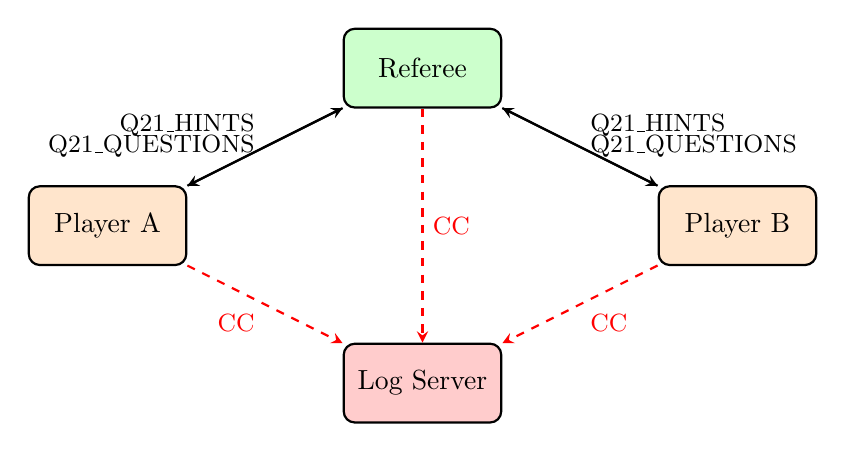
\begin{tikzpicture}[
    actor/.style={draw, thick, fill=#1!20, rounded corners, minimum width=2cm, minimum height=1cm, align=center},
    arrow/.style={->, thick, >=stealth},
    ccarrow/.style={->, thick, >=stealth, dashed, red}
]
    \node[actor=green] (ref) at (0,0) {Referee};
    \node[actor=orange] (p1) at (-4,-2) {Player A};
    \node[actor=orange] (p2) at (4,-2) {Player B};
    \node[actor=red] (log) at (0,-4) {Log Server};

    % Direct messages
    \draw[arrow] (ref) -- (p1) node[midway, above left, font=\small] {Q21\_HINTS};
    \draw[arrow] (ref) -- (p2) node[midway, above right, font=\small] {Q21\_HINTS};
    \draw[arrow] (p1) -- (ref) node[midway, left, font=\small] {Q21\_QUESTIONS};
    \draw[arrow] (p2) -- (ref) node[midway, right, font=\small] {Q21\_QUESTIONS};

    % CC arrows
    \draw[ccarrow] (ref) -- (log) node[midway, right, font=\small] {CC};
    \draw[ccarrow] (p1) -- (log) node[midway, below left, font=\small] {CC};
    \draw[ccarrow] (p2) -- (log) node[midway, below right, font=\small] {CC};
\end{tikzpicture}
\end{english}
\caption{זרימת הודעות עם \en{CC} לשרת הלוג}
\label{fig:message-flow-with-cc}
\end{figure}

% =============================================================================
\needspace{6\baselineskip}
\hebrewsection{סריקת תיקיית ספאם}
\label{sec:spam-scanning}
% =============================================================================

\needspace{10\baselineskip}
\hebrewsubsection{הדרישה}

\needspace{6\baselineskip}
\begin{protocolbox}
\textbf{כל} סוכן שופט, סוכן שחקן, ומנהל הליגה \textbf{חייבים} לסרוק את תיקיית הספאם (\en{Spam}) בשלבים הראשוניים של התקשורת.

דרישה זו חלה על כל הגורמים במערכת ללא יוצא מן הכלל.
\end{protocolbox}

\needspace{4\baselineskip}
\hebrewsubsection{מתי לסרוק ספאם?}

\begin{enumerate}
    \item \textbf{בשלב הרישום} --- מיד לאחר שליחת הודעת הרישום, יש לבדוק אם התשובה הגיעה לספאם
    \item \textbf{בתחילת כל משחק} --- לפני תחילת שלב החימום (\en{Warmup})
    \item \textbf{בזמן המתנה לתגובה} --- אם לא התקבלה תגובה בזמן הצפוי
    \item \textbf{לאחר שליחת הודעה ראשונה} --- בכל תקשורת ראשונה עם גורם חדש
\end{enumerate}

\needspace{4\baselineskip}
\hebrewsubsection{סיבות לסינון כספאם}

מערכת \en{Gmail} עלולה לסנן הודעות כספאם במקרים הבאים:

\begin{itemize}
    \item חשבון חדש ששולח הודעות לראשונה
    \item הודעות עם קבצים מצורפים (\en{JSON attachments})
    \item כתובות שאינן ברשימת אנשי הקשר
    \item תבניות הודעה אוטומטיות (נשלחות על ידי קוד)
\end{itemize}

לאסטרטגיות מניעה מפורטות והמלצות להתמודדות עם סיכוני ספאם וחסימה, ראו נספח~ה' סעיף~\ref{sec:spam-risks}.

\needspace{10\baselineskip}
\begin{warningbox}[\hebtitle{אזהרה}]
הודעה שהגיעה לתיקיית הספאם ולא נקראה בזמן תיחשב כהודעה שלא התקבלה. הסוכן עלול לקבל \textbf{הפסד טכני} אם לא יגיב בזמן בגלל אי-סריקת תיקיית הספאם.
\end{warningbox}

\needspace{10\baselineskip}
\begin{implementationbox}
\textbf{המלצה למימוש:}

בקוד הסוכן, יש לכלול לוגיקה לסריקת תיקיית הספאם בנוסף לתיבת הדואר הנכנס (\en{Inbox}). ב-\en{Gmail API}, ניתן לגשת לתיקיית הספאם באמצעות התווית \en{\texttt{SPAM}}.
\end{implementationbox}

% =============================================================================
\needspace{6\baselineskip}
\hebrewsection{תקשורת בין קבוצות}
\label{sec:inter-group-communication}
% =============================================================================

\needspace{4\baselineskip}
\hebrewsubsection{כללי תקשורת בין קבוצות}

במקרים מסוימים, קבוצות יכולות לתקשר ביניהן (למשל, לבירורים או שיתוף פעולה בנושאים טכניים). כללי התקשורת:

\begin{enumerate}
    \item \textbf{שימוש בחשבון הסוכן} --- יש לשלוח הודעות \textbf{רק} מכתובת הסוכן, לא מאימייל אישי
    \item \textbf{חובת \en{CC} לשרת הלוג} --- \textbf{כל} הודעה בין קבוצות חייבת \en{CC} לשרת הלוג
    \item \textbf{תוקף הודעה} --- הודעה שנשלחת ללא \en{CC} לשרת הלוג \textbf{אינה תקפה}
    \item \textbf{תגובה מחשבון סוכן} --- תגובה מחשבון הסוכן בלבד נחשבת לתקפה
\end{enumerate}

\needspace{10\baselineskip}
\begin{warningbox}[\hebtitle{אזהרה חשובה}]
הודעות בין קבוצות שנשלחות ללא \en{CC} לשרת הלוג לא יוכרו כתקפות במקרה של מחלוקת או צורך בביקורת.
\end{warningbox}

% =============================================================================
\needspace{8\baselineskip}
\hebrewsection{הודעות הארכה ותקלות}
\label{sec:extension-malfunction-messages}
% =============================================================================

\par\needspace{4\baselineskip}
\hebrewsubsection{בקשת הארכה (\en{EXTENSION\_REQUEST})}

שחקן יכול לבקש הארכת זמן מהשופט:

\begin{fancytable}{lHHc}{הודעות בקשת הארכה}
\label{tab:extension-messages}
סוג הודעה & מאת & אל & מועד \\
\en{EXTENSION\_REQUEST} & שחקן & שופט & \en{5m} \\
\en{EXTENSION\_RESPONSE} & שופט & שחקן & -- \\
\en{EXTENSION\_APPEAL} & שחקן & מנהל & \en{5m} \\
\en{EXTENSION\_APPEAL\_RESPONSE} & מנהל & שחקן & -- \\
\end{fancytable}

\needspace{10\baselineskip}
\begin{warningbox}[\hebtitle{מגבלת הערכות מצטברות}]
שימו לב כי לא ניתן לאשר הערכות מצטברות של כלל הסוכנים במשחק מעבר ל-\num{10} דקות בכל המשחק. כלומר אם יש השהייה מכל סיבה, בין שבגין חוסר תגובה, ובין שבגין תקלה ובגין כל סיבה אחרת --- השופט לא יכול לאשר הערכה של יותר מ-\num{10} דקות במצטבר. \textbf{מודגש:} השופט חייב לאשר בקשה להערכה ובלבד שהתקבלה בהתאם להנחיות.
\end{warningbox}

\par\needspace{4\baselineskip}
\hebrewsubsection{דוגמה --- בקשת הארכה}

\begin{english}
\begin{pythonbox}[\hebtitle{בקשת הארכה}]
{
  "protocol_version": "league.v2",
  "message_type": "EXTENSION_REQUEST",
  "message_id": "...",
  "timestamp": "2026-01-16T10:30:00Z",
  "sender_id": "P-Q21G-002",
  "game_id": "0101003",
  "payload": {
    "reason": "בעיה טכנית בחיבור לרשת",
    "requested_extension_minutes": 5,
    "evidence": "screenshot_url or description"
  }
}
\end{pythonbox}
\end{english}

\par\needspace{4\baselineskip}
\hebrewsubsection{דיווח תקלה (\en{MALFUNCTION\_REPORT})}

השופט יכול לדווח על תקלה טכנית למנהל הליגה:

\begin{fancytable}{lHHc}{הודעות דיווח תקלה}
\label{tab:malfunction-messages}
סוג הודעה & מאת & אל & מועד \\
\en{MALFUNCTION\_REPORT} & שופט & מנהל & -- \\
\en{MALFUNCTION\_ACKNOWLEDGED} & מנהל & שופט & -- \\
\en{GAME\_RESTART} & מנהל & קבוצת משחק & -- \\
\en{GAME\_CANCELLED} & מנהל & קבוצת משחק & -- \\
\end{fancytable}

\par\needspace{4\baselineskip}
\hebrewsubsection{דוגמה --- דיווח תקלה}

\begin{english}
\begin{pythonbox}[\hebtitle{דיווח תקלה}]
{
  "protocol_version": "league.v2",
  "message_type": "MALFUNCTION_REPORT",
  "message_id": "...",
  "timestamp": "2026-01-16T10:25:00Z",
  "sender_id": "R-Q21G-001",
  "game_id": "0101003",
  "payload": {
    "malfunction_type": "NETWORK_ERROR",
    "description": "Unable to receive responses from Player A",
    "game_phase": "QUESTIONS_RECEIVED",
    "affected_participants": ["P-Q21G-002"],
    "timestamp_detected": "2026-01-16T10:25:00Z"
  }
}
\end{pythonbox}
\end{english}

\par\needspace{4\baselineskip}
\hebrewsubsection{תרשים היררכיית בקשות הארכה}

איור~\ref{fig:extension-hierarchy} מציג את היררכיית בקשות ההארכה.

\begin{figure}[htbp]
\centering
\begin{english}
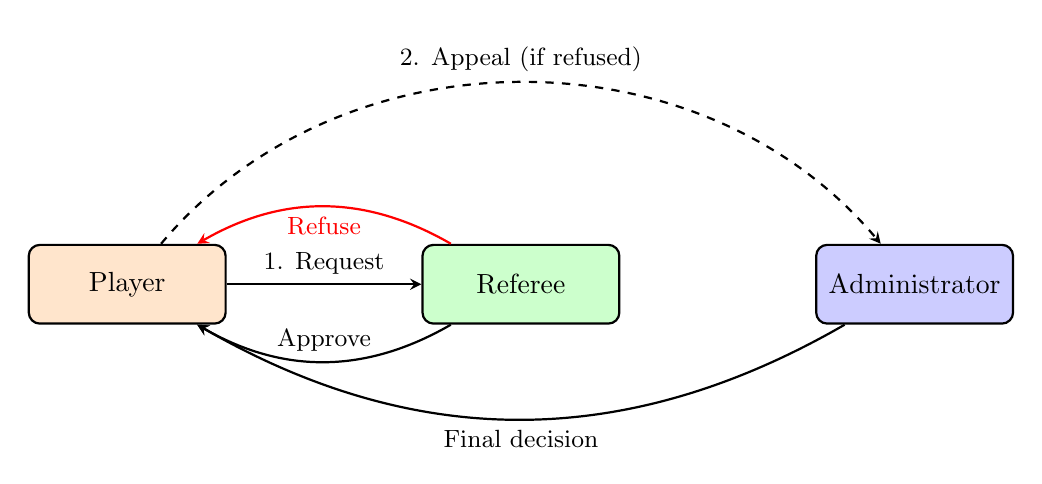
\begin{tikzpicture}[
    actor/.style={draw, thick, fill=#1!20, rounded corners, minimum width=2.5cm, minimum height=1cm, align=center},
    arrow/.style={->, thick, >=stealth},
    rejarrow/.style={->, thick, >=stealth, red}
]
    \node[actor=orange] (player) at (0,0) {Player};
    \node[actor=green] (referee) at (5,0) {Referee};
    \node[actor=blue] (admin) at (10,0) {Administrator};

    % Request flow
    \draw[arrow] (player) -- (referee) node[midway, above, font=\small] {1. Request};
    \draw[arrow, bend left=30] (referee) to node[midway, above, font=\small] {Approve} (player);
    \draw[rejarrow, bend right=30] (referee) to node[midway, below, font=\small] {Refuse} (player);

    % Appeal flow
    \draw[arrow, dashed] (player) to[bend left=50] node[midway, above, font=\small] {2. Appeal (if refused)} (admin);
    \draw[arrow, bend left=30] (admin) to node[midway, below, font=\small] {Final decision} (player);
\end{tikzpicture}
\end{english}
\caption{היררכיית בקשות הארכה --- שחקן $\rightarrow$ שופט $\rightarrow$ מנהל}
\label{fig:extension-hierarchy}
\end{figure}

% =============================================================================
\par\needspace{5\baselineskip}
\hebrewsection{ניהול מועדים}
\label{sec:deadline-management}
% =============================================================================

\par\needspace{4\baselineskip}
\hebrewsubsection{חמש קטגוריות מועדים}

\begin{fancytable}{clH}{קטגוריות מועדי תגובה}
\label{tab:deadline-categories-protocol}
מועד & קטגוריה & שימוש \\
\en{30 seconds} & \en{keep\_alive} & בדיקות זמינות \\
\en{2 minutes} & \en{critical} & הודעות בקרה \\
\en{5 minutes} & \en{game\_flow} & הזמנות, שאלות, ניחושים \\
\en{10 minutes} & \en{registration} & רישום \\
\en{24 hours} & \en{announcement} & שידורים \\
\end{fancytable}

\par\needspace{4\baselineskip}
\hebrewsubsection{תהליך אכיפת מועדים}

\begin{enumerate}
    \item כל הודעה הדורשת תגובה כוללת שדה \en{response\_deadline}
    \item המערכת מנטרת הודעות פתוחות (\en{status = 'OPEN'})
    \item בחלוף המועד ללא תגובה, הסטטוס משתנה ל-\en{REJECTED}
    \item הפסד טכני מוטל אם אין תגובה בזמן
\end{enumerate}

% =============================================================================
\par\needspace{5\baselineskip}
\hebrewsection{טיפול בתגובות מאוחרות}
\label{sec:late-response-handling}
% =============================================================================

\par\needspace{4\baselineskip}
\hebrewsubsection{הודעת \en{REJECTION\_NOTIFICATION}}

כאשר תגובה מגיעה לאחר המועד, המשתתף מקבל הודעת דחייה:

\begin{english}
\begin{pythonbox}[\hebtitle{הודעת דחייה}]
{
  "message_type": "REJECTION_NOTIFICATION",
  "correlation_id": "original-message-id",
  "payload": {
    "reason": "DEADLINE_EXCEEDED",
    "original_deadline": "2026-01-17T10:35:00Z",
    "received_at": "2026-01-17T10:37:30Z",
    "late_by_seconds": 150,
    "can_request_extension": true
  }
}
\end{pythonbox}
\end{english}

\par\needspace{4\baselineskip}
\hebrewsubsection{אפשרויות לאחר דחייה}

כאשר תגובה נדחתה, יש שתי אפשרויות:

\begin{enumerate}
    \item \textbf{בקשת הארכה} (\en{EXTENSION\_REQUEST}) --- אם הסיבה מוצדקת
    \item \textbf{קבלת הדחייה} --- ההודעה לא תיספר והמשחק ימשיך
\end{enumerate}

\needspace{8\baselineskip}
\begin{warningbox}[\hebtitle{אזהרה}]
\textbf{תגובות מאוחרות חוזרות} עלולות לגרום לפסילה מהמשחק. אם שלוש תגובות נדחו באותו משחק, הסוכן מסומן כ-\en{MALFUNCTION} והמשחק מסתיים בניקוד \en{2-2-0}.
\end{warningbox}

\par\needspace{4\baselineskip}
\hebrewsubsection{הודעת \en{ALREADY\_REJECTED\_NOTIFICATION}}

אם נשלחת תגובה להודעה שכבר נדחתה בעבר:

\begin{english}
\begin{pythonbox}[\hebtitle{הודעת דחייה כפולה}]
{
  "message_type": "ALREADY_REJECTED_NOTIFICATION",
  "correlation_id": "original-message-id",
  "payload": {
    "reason": "ALREADY_PROCESSED",
    "original_rejection_at": "2026-01-17T10:37:00Z",
    "message": "This message was already rejected. Submit extension request if needed."
  }
}
\end{pythonbox}
\end{english}

% =============================================================================
\par\needspace{5\baselineskip}
\hebrewsection{דוגמאות להודעות}
\label{sec:message-examples}
% =============================================================================

\par\needspace{4\baselineskip}
\hebrewsubsection{הודעת רמזים (\en{Q21\_HINTS})}

\begin{english}
\begin{pythonbox}[\hebtitle{הודעת רמזים}]
{
  "protocol_version": "league.v2",
  "message_type": "Q21_HINTS",
  "message_id": "550e8400-e29b-41d4-a716-446655440000",
  "timestamp": "2026-01-16T10:30:00Z",
  "sender_id": "R-Q21G-001",
  "recipient_id": "P-Q21G-002",
  "game_id": "0101003",
  "payload": {
    "description": "הפסקה עוסקת בצורה שסוכנים מתקשרים ביניהם",
    "association_topic": "טבע",
    "response_deadline": "2026-01-16T10:35:00Z"
  }
}
\end{pythonbox}
\end{english}

\par\needspace{4\baselineskip}
\hebrewsubsection{הודעת שאלות (\en{Q21\_QUESTIONS\_BATCH})}

\begin{english}
\begin{pythonbox}[\hebtitle{הודעת שאלות}]
{
  "protocol_version": "league.v2",
  "message_type": "Q21_QUESTIONS_BATCH",
  "message_id": "...",
  "timestamp": "2026-01-16T10:32:00Z",
  "sender_id": "P-Q21G-002",
  "recipient_id": "R-Q21G-001",
  "game_id": "0101003",
  "payload": {
    "questions": [
      {
        "id": 1,
        "text": "האם הפסקה עוסקת בפרוטוקול?",
        "options": ["כן", "לא", "לא ידוע", "לא רלוונטי"]
      }
      // ... 19 more questions
    ]
  }
}
\end{pythonbox}
\end{english}

\par\needspace{4\baselineskip}
\hebrewsubsection{הודעת ניחוש סופי (\en{Q21\_FINAL\_GUESS})}

\begin{english}
\begin{pythonbox}[\hebtitle{הודעת ניחוש סופי}]
{
  "protocol_version": "league.v2",
  "message_type": "Q21_FINAL_GUESS",
  "message_id": "...",
  "timestamp": "2026-01-16T10:40:00Z",
  "sender_id": "P-Q21G-002",
  "recipient_id": "R-Q21G-001",
  "game_id": "0101003",
  "payload": {
    "opening_sentence": "פרוטוקול MCP מגדיר את...",
    "sentence_reasoning": "המשפט מתאים לתיאור כי...",
    "association_word": "נחל",
    "association_variations": ["נחלים", "זרם", "זורם"],
    "association_reasoning": "תקשורת זורמת כמו נחל..."
  }
}
\end{pythonbox}
\end{english}

% =============================================================================
\par\needspace{5\baselineskip}
\hebrewsection{סיכום}
% =============================================================================

פרק זה הציג את פרוטוקול התקשורת:

\begin{itemize}
    \item שכבת תעבורה מבוססת \gmailapi{} --- פשוט ואמין
    \item מעטפת הודעה עם כותרת משותפת (\en{Shared Header})
    \item סוגי הודעות לרישום, זרימת ליגה, ומשחק
    \item חובת \en{CC} לשרת הלוג בכל הודעת משחק ובתקשורת בין קבוצות
    \item \textbf{חובת סריקת תיקיית ספאם} בשלבים הראשוניים של התקשורת --- חלה על כל הסוכנים ומנהל הליגה
    \item כללי תקשורת בין קבוצות --- שימוש בחשבון סוכן עם \en{CC} חובה
    \item הודעות הארכה ותקלות: \en{EXTENSION\_REQUEST}, \en{MALFUNCTION\_REPORT}
    \item היררכיית ערעורים: שחקן $\rightarrow$ שופט $\rightarrow$ מנהל
    \item חמש קטגוריות מועדים עם אכיפה
\end{itemize}

בפרק הבא נעסוק במימוש המעשי של הסוכנים.

\end{document}
